\subsection{Package \lstinline!cryptocast.crypto!}
This package provides basic primitives for working with broadcast encryption protocols
 and useful utilities for working with polynomials and elliptic curves over fields, which
 is necessary to implement the Naor-Pinkas scheme.

\noindent\begin{minipage}[t]{5cm}
\vspace{0.3em}
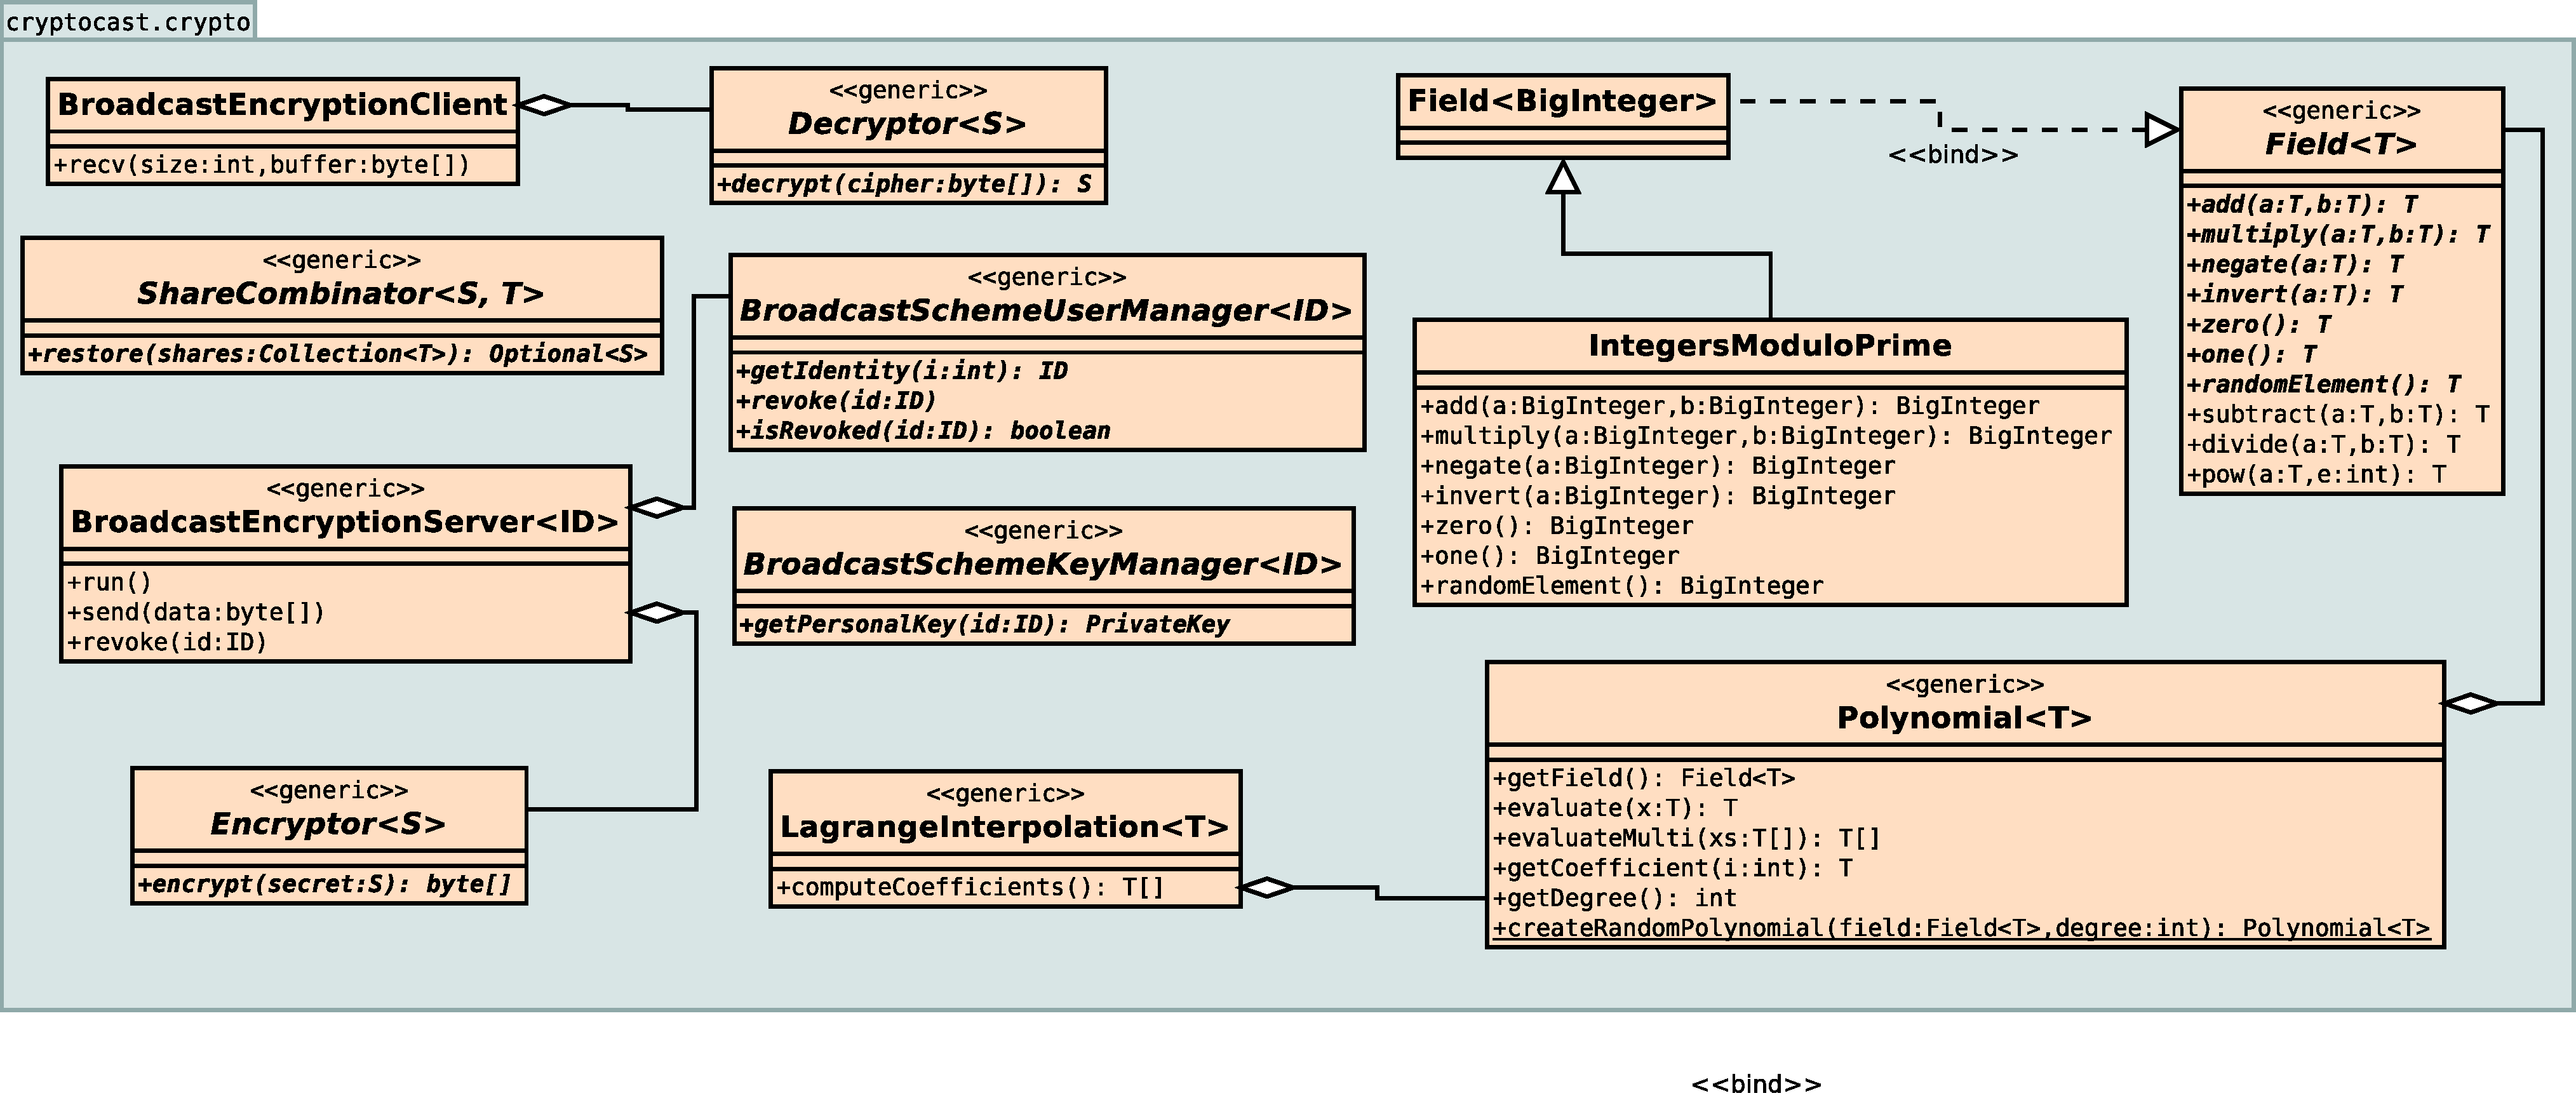
\includegraphics[width=450px]{class_diagrams/cryptocast_crypto.pdf}
\end{minipage}

\subsubsection{Class \lstinline|InsufficientInformationError|}
An exception that represents an error due to missing information (for
 example, in a threshold scheme). \\
\noindent\begin{minipage}[t]{5cm}
\vspace{0.3em}
\hspace*{2em}
\begin{tikzpicture}
\umlclass[]{InsufficientInformationError}{

}{

}
\end{tikzpicture}
\vspace{0.3em}
\end{minipage}



\textbf{\sffamily Superclasses and Interfaces}
\begin{itemize}
\item \lstinline|cryptocast.crypto.DecryptionError|
\end{itemize}


\textbf{\sffamily Constructors}
\begin{itemize}
\item \lstinline|public| \lstinline|InsufficientInformationError|\lstinline|(String msg)|\\ \\[-0.6em]
Creates a new insufficient error with the given message.
\begin{itemize}
\item \lstinline|msg|: The error message.
\end{itemize}



\end{itemize}


\subsubsection{Class \lstinline|LagrangeInterpolation<T>|}
Represents the context needed to quickly perform a Lagrange interpolation of
 the values $P_i(0)$ of arbitrarily many polnomials $P_i$.
 Given a set of points ${x_1, ..., x_n}$, the state needed to do this is the
 values $c_i = \prod_{i \neq j} \frac{x_j}{x_j - x_i}$. \\
\noindent\begin{minipage}[t]{5cm}
\vspace{0.3em}
\hspace*{2em}
\begin{tikzpicture}
\umlclass[]{LagrangeInterpolation<T>}{

}{
+ getCoefficients() : Map<T, T> \\
+ getField() : Field<T> \\
\umlstatic{+ fromXs(field : Field<T>, xs : ImmutableList<T>, numThreads : int) : LagrangeInterpolation<T>} \\
\umlstatic{+ fromXs(field : Field<T>, xs : ImmutableList<T>) : LagrangeInterpolation<T>} \\
+ interpolateP0(evaluate : Function<?, T, T>) : T \\
+ interpolateP0(dataPoints : Map<T, T>) : T \\
+ setXs(xs : Set<T>) \\
+ addXs(newXs : Set<T>) \\
+ removeXs(removeXs : Set<T>) \\
+ addX(newX : T) \\
+ removeX(removedX : T) \\
\umlstatic{+ computeCoefficients(field : Field<T>, xs : ImmutableList<T>, numThreads : int) : ImmutableList<T>} \\
+ equals(other\_ : Object) : boolean
}
\end{tikzpicture}
\vspace{0.3em}
\end{minipage}

\begin{itemize}
\item \lstinline|<T>|: The type of items of the polynomial over a field.
\end{itemize}


\textbf{\sffamily Superclasses and Interfaces}
\begin{itemize}
\item \lstinline|java.io.Serializable|
\end{itemize}


\textbf{\sffamily Constructors}
\begin{itemize}
\item \lstinline|public| \lstinline|LagrangeInterpolation|\lstinline|(Field<T> field)|\\ \\[-0.6em]
Creates an instance of this class.
\begin{itemize}
\item \lstinline|field|: The field over which the interpolation is constructed.
\end{itemize}



\item \lstinline|public| \lstinline|LagrangeInterpolation|\lstinline|(Field<T> field, Map<T, T> coefficients)|\\ \\[-0.6em]
Creates an instance of this class.
\begin{itemize}
\item \lstinline|field|: The field over which the interpolation is constructed.
\item \lstinline|coefficients|: The initial lagrange coefficients, which is a map
 $T \to T$ that assigns places $x_i$ their coefficients
 $c_i = \prod_{i \neq j} \frac{x_j}{x_j - x_i}$.
\end{itemize}



\end{itemize}


\textbf{\sffamily Methods}
\begin{itemize}
\item \lstinline|public Map<T, T>| \lstinline|getCoefficients|\lstinline|()|\\ \\[-0.6em]
\emph{Returns:} The Lagrange coefficients. This is a map $T \to T$ that assigns places $x_i$
 their coefficients
 $c_i = \prod_{i \neq j} \frac{x_j}{x_j - x_i}$.



\item \lstinline|public Field<T>| \lstinline|getField|\lstinline|()|\\ \\[-0.6em]
\emph{Returns:} The field of the interpolation.



\item \lstinline|public static LagrangeInterpolation<T>| \lstinline|fromXs|\lstinline|(Field<T> field, ImmutableList<T> xs, int numThreads)|\\ \\[-0.6em]
Creates an instance of this class from a list of points.
\begin{itemize}
\item \lstinline|field|: The field over which the interpolation is constructed.
\item \lstinline|xs|: The list of points $x_i$.
\item \lstinline|numThreads|: The number of threads for concurrent evaluation.
\end{itemize}

\emph{Returns:} An instance of this class from a list of points.

\item \lstinline|public static LagrangeInterpolation<T>| \lstinline|fromXs|\lstinline|(Field<T> field, ImmutableList<T> xs)|\\ \\[-0.6em]
Creates an instance of this class from a list of points using a default number of threads.
\begin{itemize}
\item \lstinline|field|: The field over which the polynomial is constructed.
\item \lstinline|xs|: The list of points.
\end{itemize}

\emph{Returns:} An instance of this class from a list of points using default number of threads.

\item \lstinline|public T| \lstinline|interpolateP0|\lstinline|(Function<?, T, T> evaluate)|\\ \\[-0.6em]
Interpolates $P(0)$ using the function $P$ to compute the values
 $P(x_i)$.
\begin{itemize}
\item \lstinline|evaluate|: The function that evaluates the polynomial $P$ at the
 given points.
\end{itemize}

\emph{Returns:} The interpolation result.

\item \lstinline|public T| \lstinline|interpolateP0|\lstinline|(Map<T, T> dataPoints)|\\ \\[-0.6em]
Interpolates $P(0)$ where $P$ is the Lagrange polynomial of
 the given data point.
\begin{itemize}
\item \lstinline|dataPoints|: The data points.
\end{itemize}

\emph{Returns:} The interpolation result.

\item \lstinline|public void| \lstinline|setXs|\lstinline|(Set<T> xs)|\\ \\[-0.6em]
Sets the set ${x_1, ..., x_n}$.
\begin{itemize}
\item \lstinline|xs|: The set of points.
\end{itemize}



\item \lstinline|public void| \lstinline|addXs|\lstinline|(Set<T> newXs)|\\ \\[-0.6em]
Adds the set ${x_{n+1}, ..., x_{n+m}}$ to the interal set of points.
\begin{itemize}
\item \lstinline|newXs|: The new points.
\end{itemize}



\item \lstinline|public void| \lstinline|removeXs|\lstinline|(Set<T> removeXs)|\\ \\[-0.6em]
Removes the set ${x_{n-m}, ..., x_n}$ from the internal set of points.
\begin{itemize}
\item \lstinline|removeXs|: The points to remove
\end{itemize}



\item \lstinline|public void| \lstinline|addX|\lstinline|(T newX)|\\ \\[-0.6em]
Adds a point to the internal set of points
\begin{itemize}
\item \lstinline|newX|: The point to add.
\end{itemize}



\item \lstinline|public void| \lstinline|removeX|\lstinline|(T removedX)|\\ \\[-0.6em]
Removes a point from the internal set of points.
\begin{itemize}
\item \lstinline|removedX|: The point to remove.
\end{itemize}



\item \lstinline|public static ImmutableList<T>| \lstinline|computeCoefficients|\lstinline|(Field<T> field, ImmutableList<T> xs, int numThreads)|\\ \\[-0.6em]
Computes the langrange coefficients for a given list of points.
 Uses native acceleration if available.
\begin{itemize}
\item \lstinline|field|: The field
\item \lstinline|xs|: The list $x_i$
\item \lstinline|numThreads|: the number of threds to use for parallelisation
\end{itemize}

\emph{Returns:} The Lagrange coefficients $c_i$,
         where $c_i = \prod_{j \neq i} \frac{x_j}{x_j - x_i}$

\item \lstinline|public boolean| \lstinline|equals|\lstinline|(Object other_)| \\[-0.6em]




\end{itemize}

\subsubsection{Class \lstinline|DynamicCipherOutputStream|}
Represents an output stream wrapper that encrypts its data on-the-fly using
 AES/CBC with a session key that can be switched at any time during
 transmission.
 This stream uses a message-based communication channel. \\
\noindent\begin{minipage}[t]{5cm}
\vspace{0.3em}
\hspace*{2em}
\begin{tikzpicture}
\umlclass[]{DynamicCipherOutputStream}{

}{
\umlstatic{+ start(inner : MessageOutChannel, keyBits : int, enc : Encryptor<byte[]>) : DynamicCipherOutputStream} \\
+ updateKey() \\
+ reinitializeCipher() \\
+ write(data : byte[], offset : int, len : int) \\
+ write(b : int) \\
+ close()
}
\end{tikzpicture}
\vspace{0.3em}
\end{minipage}



\textbf{\sffamily Superclasses and Interfaces}
\begin{itemize}
\item \lstinline|java.io.OutputStream|
\end{itemize}


\textbf{\sffamily Constructors}
\begin{itemize}
\item \lstinline|private| \lstinline|DynamicCipherOutputStream|\lstinline|(MessageOutChannel inner, int keyBits, Encryptor<byte[]> enc)| \\[-0.6em]




\end{itemize}


\textbf{\sffamily Methods}
\begin{itemize}
\item \lstinline|public static DynamicCipherOutputStream| \lstinline|start|\lstinline|(MessageOutChannel inner, int keyBits, Encryptor<byte[]> enc)|\\ \\[-0.6em]
Creates a new dynamic cipher output stream with the given values.
\begin{itemize}
\item \lstinline|inner|: The underlying message-based communication channel.
\item \lstinline|keyBits|: The width of the symmetric key (128, 192 or 256 bits).
 For 192 or 256 bits, the Strong Cryptography Jurasdiction JVM additions
 must be installed.
\item \lstinline|enc|: The strategy for encrypting the session key in key update
 messages.
\end{itemize}

\emph{Returns:} a new dynamic cipher output stream.

\item \lstinline|public void| \lstinline|updateKey|\lstinline|()|\\ \\[-0.6em]
Updates the key. Will send a control message to the other side and
 switch the cipher.



\item \lstinline|public void| \lstinline|reinitializeCipher|\lstinline|()|\\ \\[-0.6em]
Reinitializes the cipher. Will broadcast the old session key to the other
 side. If the session key is the same as last time, it will *not* be
 reencrypted. The cached version will be used.



\item \lstinline|public void| \lstinline|write|\lstinline|(byte[] data, int offset, int len)| \\[-0.6em]




\item \lstinline|public void| \lstinline|write|\lstinline|(int b)| \\[-0.6em]




\item \lstinline|public void| \lstinline|close|\lstinline|()| \\[-0.6em]




\end{itemize}

\subsubsection{Class \lstinline|PolynomialMultiEvaluation|}
Used to evaluate a polynomial at multiple points. A native function is used, if n
 is bigger than a specific threshold. \\
\noindent\begin{minipage}[t]{5cm}
\vspace{0.3em}
\hspace*{2em}
\begin{tikzpicture}
\umlclass[]{PolynomialMultiEvaluation}{

}{
+ evaluate(poly : Polynomial<BigInteger>) : ImmutableList<BigInteger>
}
\end{tikzpicture}
\vspace{0.3em}
\end{minipage}




\textbf{\sffamily Constructors}
\begin{itemize}
\item \lstinline|public| \lstinline|PolynomialMultiEvaluation|\lstinline|(List<BigInteger> xs, int numThreads, int chunkSize)|\\ \\[-0.6em]
Creates an instance of the polynomial multi evaluation.
\begin{itemize}
\item \lstinline|xs|: The list of the polynomial points.
\item \lstinline|numThreads|: The number of threads for the concurrent native function.
\item \lstinline|chunkSize|: The chunk size for each thread.
\end{itemize}



\item \lstinline|public| \lstinline|PolynomialMultiEvaluation|\lstinline|(List<BigInteger> xs)|\\ \\[-0.6em]
Creates an instance of the polynomial multi evaluation.
\begin{itemize}
\item \lstinline|xs|: The list of the polynomial points.
\end{itemize}



\end{itemize}


\textbf{\sffamily Methods}
\begin{itemize}
\item \lstinline|public ImmutableList<BigInteger>| \lstinline|evaluate|\lstinline|(Polynomial<BigInteger> poly)|\\ \\[-0.6em]
Evaluates the polynomial.
\begin{itemize}
\item \lstinline|poly|: The polynomial to evaluate.
\end{itemize}

\emph{Returns:} The evaluation result.

\end{itemize}

\subsubsection{Class \lstinline|EllipticCurveGroup<T, P, C>|}
Represents the cyclic group structure of the set of points $kG$ generated
 by a generator $G$, which is a point on an elliptic curve. \\
\noindent\begin{minipage}[t]{5cm}
\vspace{0.3em}
\hspace*{2em}
\begin{tikzpicture}
\umlclass[]{EllipticCurveGroup<T, P, C>}{

}{
+ getCurve() : C \\
+ combine(a : P, b : P) : P \\
+ twice(a : P) : P \\
+ pow(a : P, k : BigInteger) : P \\
+ invert(a : P) : P \\
+ identity() : P \\
+ multiexp(bases : List<P>, exponents : List<BigInteger>) : P \\
\umlstatic{+ getSecp160R1() : EllipticCurveGroup<BigInteger, Point, EllipticCurveOverFp>}
}
\end{tikzpicture}
\vspace{0.3em}
\end{minipage}

\begin{itemize}
\item \lstinline|<T>|: The type of coordinates of the curves points.
\item \lstinline|<P>|: The type of points of the curve.
\item \lstinline|<C>|: The type of the curve.
\end{itemize}


\textbf{\sffamily Superclasses and Interfaces}
\begin{itemize}
\item \lstinline|cryptocast.crypto.CyclicGroupOfPrimeOrder<P>|
\item \lstinline|java.io.Serializable|
\end{itemize}


\textbf{\sffamily Constructors}
\begin{itemize}
\item \lstinline|public| \lstinline|EllipticCurveGroup|\lstinline|(C curve, P basePoint, BigInteger basePointOrder)|\\ \\[-0.6em]
Generates a group from the given parameters.
\begin{itemize}
\item \lstinline|curve|: The elliptic curve.
\item \lstinline|basePoint|: The generator point.
\item \lstinline|basePointOrder|: The order of the generator point.
\end{itemize}



\end{itemize}


\textbf{\sffamily Methods}
\begin{itemize}
\item \lstinline|public C| \lstinline|getCurve|\lstinline|()|\\ \\[-0.6em]
\emph{Returns:} The curve.



\item \lstinline|public P| \lstinline|combine|\lstinline|(P a, P b)| \\[-0.6em]




\item \lstinline|public P| \lstinline|twice|\lstinline|(P a)| \\[-0.6em]




\item \lstinline|public P| \lstinline|pow|\lstinline|(P a, BigInteger k)| \\[-0.6em]




\item \lstinline|public P| \lstinline|invert|\lstinline|(P a)| \\[-0.6em]




\item \lstinline|public P| \lstinline|identity|\lstinline|()| \\[-0.6em]




\item \lstinline|public P| \lstinline|multiexp|\lstinline|(List<P> bases, List<BigInteger> exponents)|\\ \\[-0.6em]
Uses Shamir's trick to get much better performance. Uses \lstinline|List.subList|, so you'd
 better give it \lstinline|ImmutableLists|.



\item \lstinline|public static EllipticCurveGroup<BigInteger, Point, EllipticCurveOverFp>| \lstinline|getSecp160R1|\lstinline|()| \\[-0.6em]




\end{itemize}

\subsubsection{Class \lstinline|CryptoUtils|}
Simple helper functions for symmetric encryption/decryption and hashing. \\
\noindent\begin{minipage}[t]{5cm}
\vspace{0.3em}
\hspace*{2em}
\begin{tikzpicture}
\umlclass[]{CryptoUtils}{

}{
\umlstatic{+ encrypt(plain : byte[], key : byte[]) : byte[]} \\
\umlstatic{+ decrypt(cipher : byte[], key : byte[]) : byte[]} \\
\umlstatic{+ encryptAndHash(plain : byte[], key : byte[]) : byte[]} \\
\umlstatic{+ decryptAndHash(cipher : byte[], key : byte[]) : byte[]} \\
\umlstatic{+ sha256(input : byte[]) : byte[]}
}
\end{tikzpicture}
\vspace{0.3em}
\end{minipage}





\textbf{\sffamily Methods}
\begin{itemize}
\item \lstinline|public static byte[]| \lstinline|encrypt|\lstinline|(byte[] plain, byte[] key)|\\ \\[-0.6em]
Encrypts a plain text using AES-128 with the given key.
\begin{itemize}
\item \lstinline|plain|: The plain text.
\item \lstinline|key|: The key.
\end{itemize}

\emph{Returns:} The cipher text.

\item \lstinline|public static byte[]| \lstinline|decrypt|\lstinline|(byte[] cipher, byte[] key)|\\ \\[-0.6em]
Decrypts a cipher text using AES-128 with the given key.
\begin{itemize}
\item \lstinline|cipher|: The cipher text.
\item \lstinline|key|: The key.
\end{itemize}

\emph{Returns:} The plain text.

\item \lstinline|public static byte[]| \lstinline|encryptAndHash|\lstinline|(byte[] plain, byte[] key)|\\ \\[-0.6em]
Encrypts a plain text along with its SHA-256 hash using AES-128 with the given key.
\begin{itemize}
\item \lstinline|plain|: The plain text.
\item \lstinline|key|: The key.
\end{itemize}

\emph{Returns:} The cipher text.

\item \lstinline|public static byte[]| \lstinline|decryptAndHash|\lstinline|(byte[] cipher, byte[] key)|\\ \\[-0.6em]
Decrypts a cipher text that was encrypted using \lstinline|encryptAndHash|
 using the given key and verify the integrity of the plain text by
 examining the supplied hash.
\begin{itemize}
\item \lstinline|cipher|: The cipher text.
\item \lstinline|key|: The key.
\end{itemize}

\emph{Returns:} The plain text.

\item \lstinline|public static byte[]| \lstinline|sha256|\lstinline|(byte[] input)|\\ \\[-0.6em]
Computes the SHA-256 hash of the given input.
\begin{itemize}
\item \lstinline|input|: The input data
\end{itemize}

\emph{Returns:} The hash.

\end{itemize}

\subsubsection{Class \lstinline|IntegersModuloPrime|}
The field $GF(p)$ of integers modulo a prime $p > 2$. \\
\noindent\begin{minipage}[t]{5cm}
\vspace{0.3em}
\hspace*{2em}
\begin{tikzpicture}
\umlclass[]{IntegersModuloPrime}{

}{
+ reduce(a : BigInteger) : BigInteger \\
+ getP() : BigInteger \\
+ add(a : BigInteger, b : BigInteger) : BigInteger \\
+ multiply(a : BigInteger, b : BigInteger) : BigInteger \\
+ negate(a : BigInteger) : BigInteger \\
+ invert(a : BigInteger) : BigInteger \\
+ zero() : BigInteger \\
+ one() : BigInteger \\
+ two() : BigInteger \\
+ three() : BigInteger \\
+ four() : BigInteger \\
+ subtract(a : BigInteger, b : BigInteger) : BigInteger \\
+ pow(a : BigInteger, e : BigInteger) : BigInteger \\
+ randomElement(rnd : Random) : BigInteger \\
+ isZero(a : BigInteger) : boolean \\
+ equals(other : Object) : boolean \\
+ sqrt(a : BigInteger) : Optional<BigInteger>
}
\end{tikzpicture}
\vspace{0.3em}
\end{minipage}



\textbf{\sffamily Superclasses and Interfaces}
\begin{itemize}
\item \lstinline|cryptocast.crypto.Field<BigInteger>|
\item \lstinline|java.io.Serializable|
\end{itemize}


\textbf{\sffamily Constructors}
\begin{itemize}
\item \lstinline|public| \lstinline|IntegersModuloPrime|\lstinline|(BigInteger p)|\\ \\[-0.6em]
Initializes the field.
\begin{itemize}
\item \lstinline|p|: A prime number (must not be $2$)
\end{itemize}



\end{itemize}


\textbf{\sffamily Methods}
\begin{itemize}
\item \lstinline|public BigInteger| \lstinline|reduce|\lstinline|(BigInteger a)|\\ \\[-0.6em]
Reduces an integer $a < p^2$ modulo $p$.
\begin{itemize}
\item \lstinline|a|: ($a < p^2$)
\end{itemize}

\emph{Returns:} $a \bmod{p}$

\item \lstinline|public BigInteger| \lstinline|getP|\lstinline|()|\\ \\[-0.6em]
\emph{Returns:} $p$



\item \lstinline|public BigInteger| \lstinline|add|\lstinline|(BigInteger a, BigInteger b)| \\[-0.6em]




\item \lstinline|public BigInteger| \lstinline|multiply|\lstinline|(BigInteger a, BigInteger b)| \\[-0.6em]




\item \lstinline|public BigInteger| \lstinline|negate|\lstinline|(BigInteger a)| \\[-0.6em]




\item \lstinline|public BigInteger| \lstinline|invert|\lstinline|(BigInteger a)| \\[-0.6em]




\item \lstinline|public BigInteger| \lstinline|zero|\lstinline|()| \\[-0.6em]




\item \lstinline|public BigInteger| \lstinline|one|\lstinline|()| \\[-0.6em]




\item \lstinline|public BigInteger| \lstinline|two|\lstinline|()| \\[-0.6em]




\item \lstinline|public BigInteger| \lstinline|three|\lstinline|()| \\[-0.6em]




\item \lstinline|public BigInteger| \lstinline|four|\lstinline|()| \\[-0.6em]




\item \lstinline|public BigInteger| \lstinline|subtract|\lstinline|(BigInteger a, BigInteger b)| \\[-0.6em]




\item \lstinline|public BigInteger| \lstinline|pow|\lstinline|(BigInteger a, BigInteger e)| \\[-0.6em]




\item \lstinline|public BigInteger| \lstinline|randomElement|\lstinline|(Random rnd)| \\[-0.6em]




\item \lstinline|public boolean| \lstinline|isZero|\lstinline|(BigInteger a)| \\[-0.6em]




\item \lstinline|public boolean| \lstinline|equals|\lstinline|(Object other)| \\[-0.6em]




\item \lstinline|public Optional<BigInteger>| \lstinline|sqrt|\lstinline|(BigInteger a)| \\[-0.6em]




\end{itemize}

\subsubsection{Class \lstinline|EllipticCurve.AffinePoint<T>|}
Represents a point on the elliptic curve that is not the identity
 element. \\
\noindent\begin{minipage}[t]{5cm}
\vspace{0.3em}
\hspace*{2em}
\begin{tikzpicture}
\umlclass[]{EllipticCurve.AffinePoint<T>}{

}{
+ getX() : T \\
+ getY() : T \\
+ equals(other : Object) : boolean
}
\end{tikzpicture}
\vspace{0.3em}
\end{minipage}

\begin{itemize}
\item \lstinline|<T>|: The type of the coordinates
\end{itemize}



\textbf{\sffamily Constructors}
\begin{itemize}
\item \lstinline|public| \lstinline|EllipticCurve.AffinePoint|\lstinline|(T x, T y)|\\ \\[-0.6em]
Creates an instance.
\begin{itemize}
\item \lstinline|x|: The first coordinate of the point.
\item \lstinline|y|: The second coordinate of the point.
\end{itemize}



\end{itemize}


\textbf{\sffamily Methods}
\begin{itemize}
\item \lstinline|public T| \lstinline|getX|\lstinline|()|\\ \\[-0.6em]
\emph{Returns:} The first coordinate of the point.



\item \lstinline|public T| \lstinline|getY|\lstinline|()|\\ \\[-0.6em]
\emph{Returns:} The second coordinate of the point.



\item \lstinline|public boolean| \lstinline|equals|\lstinline|(Object other)| \\[-0.6em]




\end{itemize}

\subsubsection{Class \lstinline|Polynomial<T>|}
A polynomial $P$ over a field. \\
\noindent\begin{minipage}[t]{5cm}
\vspace{0.3em}
\hspace*{2em}
\begin{tikzpicture}
\umlclass[]{Polynomial<T>}{

}{
+ getField() : Field<T> \\
+ evaluate(x : T) : T \\
+ getEvaluator() : Function<T, T> \\
+ evaluateMulti(xs : ImmutableList<T>) : ImmutableList<T> \\
+ getCoefficients() : ImmutableList<T> \\
+ getSize() : int \\
+ getDegree() : int \\
\umlstatic{+ createRandomPolynomial(rnd : Random, field : Field<T>, size : int) : Polynomial<T>} \\
+ equals(other\_ : Object) : boolean \\
+ toString() : String
}
\end{tikzpicture}
\vspace{0.3em}
\end{minipage}

\begin{itemize}
\item \lstinline|<T>|: The type of the field's elements
\end{itemize}


\textbf{\sffamily Superclasses and Interfaces}
\begin{itemize}
\item \lstinline|java.io.Serializable|
\end{itemize}


\textbf{\sffamily Constructors}
\begin{itemize}
\item \lstinline|public| \lstinline|Polynomial|\lstinline|(Field<T> field, List<T> coefficients)|\\ \\[-0.6em]
Initializes a polynomial.
\begin{itemize}
\item \lstinline|field|: An instance of the field over which the polynomial is formed.
\item \lstinline|coefficients|: The coefficients $c_i$ of the polynomial ($0 \leq i \leq n$).
 The polynomial is defined as $P(x) := \sum_{i=0}^n c_i x^i = c_0 + c_1
 x + ... + c_n x^n$.
\end{itemize}



\end{itemize}


\textbf{\sffamily Methods}
\begin{itemize}
\item \lstinline|public Field<T>| \lstinline|getField|\lstinline|()|\\ \\[-0.6em]
\emph{Returns:} The field associated with this polynomial.



\item \lstinline|public T| \lstinline|evaluate|\lstinline|(T x)|\\ \\[-0.6em]
Evaluates the polynomial at a single point $x$.
\begin{itemize}
\item \lstinline|x|: The point
\end{itemize}

\emph{Returns:} $P(x)$

\item \lstinline|public Function<T, T>| \lstinline|getEvaluator|\lstinline|()|\\ \\[-0.6em]
\emph{Returns:} A function evaluating this polynomial.



\item \lstinline|public ImmutableList<T>| \lstinline|evaluateMulti|\lstinline|(ImmutableList<T> xs)|\\ \\[-0.6em]
Evaluates the polynomial at multiple points using a naive algorithm.
\begin{itemize}
\item \lstinline|xs|: The points $x_i$ to evaluate
\end{itemize}

\emph{Returns:} The array a defined by $a_i := P(x_i)$.

\item \lstinline|public ImmutableList<T>| \lstinline|getCoefficients|\lstinline|()|\\ \\[-0.6em]
Returns the coefficients list of this polynomial.

\emph{Returns:} $c_i$

\item \lstinline|public int| \lstinline|getSize|\lstinline|()|\\ \\[-0.6em]
\emph{Returns:} The size of the polynomial (degree plus one or 0 if the polynomial
 is constant zero).



\item \lstinline|public int| \lstinline|getDegree|\lstinline|()|\\ \\[-0.6em]
\emph{Returns:} The degree of the polynomial or -1 if the polynomial is zero.



\item \lstinline|public static Polynomial<T>| \lstinline|createRandomPolynomial|\lstinline|(Random rnd, Field<T> field, int size)|\\ \\[-0.6em]
Generates a random polynomial over a field.
\begin{itemize}
\item \lstinline|rnd|: The source of randomness
\item \lstinline|field|: An instance of the field over which the polynomial is formed.
\item \lstinline|size|: The size of the polynomial (see \lstinline|getSize|)
\end{itemize}

\emph{Returns:} The generated polynomial

\item \lstinline|public boolean| \lstinline|equals|\lstinline|(Object other_)| \\[-0.6em]




\item \lstinline|public String| \lstinline|toString|\lstinline|()| \\[-0.6em]




\end{itemize}

\subsubsection{Class \lstinline|EllipticCurveOverFp|}
An elliptic curve over $GF(p)$ where $p$ is prime. \\
\noindent\begin{minipage}[t]{5cm}
\vspace{0.3em}
\hspace*{2em}
\begin{tikzpicture}
\umlclass[]{EllipticCurveOverFp}{

}{
+ isInfinity(point : Point) : boolean \\
+ getInfinity() : Point \\
+ getA() : BigInteger \\
+ getB() : BigInteger \\
+ getPoint(x : BigInteger, y : BigInteger) : Point \\
+ getField() : IntegersModuloPrime \\
+ negate(a : Point) : Point \\
+ add(p : Point, q : Point) : Point \\
+ twice(p : Point) : Point \\
+ multiply(p : Point, k : BigInteger) : Point \\
+ compress(p : Point) : CompressedPoint \\
+ uncompress(p : CompressedPoint) : Point \\
+ getAffineCoords(p : Point) : Optional<AffinePoint<BigInteger>, BigInteger> \\
+ subtract(a : Point, b : Point) : Point
}
\end{tikzpicture}
\vspace{0.3em}
\end{minipage}



\textbf{\sffamily Superclasses and Interfaces}
\begin{itemize}
\item \lstinline|cryptocast.crypto.EllipticCurve<BigInteger, Point>|
\item \lstinline|java.io.Serializable|
\end{itemize}


\textbf{\sffamily Constructors}
\begin{itemize}
\item \lstinline|public| \lstinline|EllipticCurveOverFp|\lstinline|(IntegersModuloPrime field, BigInteger a, BigInteger b)| \\[-0.6em]

\begin{itemize}
\item \lstinline|field|: The field $GF(p)$
\item \lstinline|a|: The coefficient $a$ of the curve.
\item \lstinline|b|: The coefficient $b$ of the curve.
\end{itemize}



\end{itemize}


\textbf{\sffamily Methods}
\begin{itemize}
\item \lstinline|public boolean| \lstinline|isInfinity|\lstinline|(Point point)| \\[-0.6em]




\item \lstinline|public Point| \lstinline|getInfinity|\lstinline|()| \\[-0.6em]




\item \lstinline|public BigInteger| \lstinline|getA|\lstinline|()| \\[-0.6em]




\item \lstinline|public BigInteger| \lstinline|getB|\lstinline|()| \\[-0.6em]




\item \lstinline|public Point| \lstinline|getPoint|\lstinline|(BigInteger x, BigInteger y)| \\[-0.6em]




\item \lstinline|public IntegersModuloPrime| \lstinline|getField|\lstinline|()| \\[-0.6em]




\item \lstinline|public Point| \lstinline|negate|\lstinline|(Point a)| \\[-0.6em]




\item \lstinline|public Point| \lstinline|add|\lstinline|(Point p, Point q)| \\[-0.6em]




\item \lstinline|public Point| \lstinline|twice|\lstinline|(Point p)| \\[-0.6em]




\item \lstinline|public Point| \lstinline|multiply|\lstinline|(Point p, BigInteger k)| \\[-0.6em]




\item \lstinline|public CompressedPoint| \lstinline|compress|\lstinline|(Point p)|\\ \\[-0.6em]
\emph{Returns:} The compressed represntation of $p$.
\begin{itemize}
\item \lstinline|p|: a point
\end{itemize}



\item \lstinline|public Point| \lstinline|uncompress|\lstinline|(CompressedPoint p)|\\ \\[-0.6em]
\emph{Returns:} The uncompressed representation of $p$.
\begin{itemize}
\item \lstinline|p|: a compressed point
\end{itemize}



\item \lstinline|public Optional<AffinePoint<BigInteger>, BigInteger>| \lstinline|getAffineCoords|\lstinline|(Point p)| \\[-0.6em]




\item \lstinline|public Point| \lstinline|subtract|\lstinline|(Point a, Point b)| \\[-0.6em]




\end{itemize}

\subsubsection{Class \lstinline|EllipticCurveOverFp.Point|}
A point on the curve. \\
\noindent\begin{minipage}[t]{5cm}
\vspace{0.3em}
\hspace*{2em}
\begin{tikzpicture}
\umlclass[]{EllipticCurveOverFp.Point}{

}{
+ equals(other\_ : Object) : boolean
}
\end{tikzpicture}
\vspace{0.3em}
\end{minipage}



\textbf{\sffamily Superclasses and Interfaces}
\begin{itemize}
\item \lstinline|java.io.Serializable|
\end{itemize}


\textbf{\sffamily Constructors}
\begin{itemize}
\item \lstinline|private| \lstinline|EllipticCurveOverFp.Point|\lstinline|(BigInteger jx, BigInteger jy, BigInteger jz, EllipticCurveOverFp curve)| \\[-0.6em]




\end{itemize}


\textbf{\sffamily Methods}
\begin{itemize}
\item \lstinline|public boolean| \lstinline|equals|\lstinline|(Object other_)| \\[-0.6em]




\end{itemize}

\subsubsection{Class \lstinline|EllipticCurveOverFp.CompressedPoint|}
A representation of a point compressed to the $x$ coordinate. \\
\noindent\begin{minipage}[t]{5cm}
\vspace{0.3em}
\hspace*{2em}
\begin{tikzpicture}
\umlclass[]{EllipticCurveOverFp.CompressedPoint}{

}{
+ getX() : BigInteger \\
+ getInfo() : byte
}
\end{tikzpicture}
\vspace{0.3em}
\end{minipage}




\textbf{\sffamily Constructors}
\begin{itemize}
\item \lstinline|public| \lstinline|EllipticCurveOverFp.CompressedPoint|\lstinline|(BigInteger x, byte info)| \\[-0.6em]




\end{itemize}


\textbf{\sffamily Methods}
\begin{itemize}
\item \lstinline|public BigInteger| \lstinline|getX|\lstinline|()| \\[-0.6em]




\item \lstinline|public byte| \lstinline|getInfo|\lstinline|()| \\[-0.6em]




\end{itemize}

\subsubsection{Class \lstinline|CyclicGroupOfPrimeOrder<T>|}
Represents a cyclic group $(G, \otimes)$ of prime order $q$ over a subset
 $G$ of the values of type T, generated by $g$.
 Let $e$ denote the identity element of $G$ and $x^{-1}$ the inverse of $x$. \\
\noindent\begin{minipage}[t]{5cm}
\vspace{0.3em}
\hspace*{2em}
\begin{tikzpicture}
\umlclass[type=abstract]{CyclicGroupOfPrimeOrder<T>}{

}{
+ getGenerator() : T \\
+ getPowerOfG(k : BigInteger) : T \\
+ getOrder() : BigInteger \\
+ getFieldModOrder() : IntegersModuloPrime \\
\umlvirt{+ combine(a : T, b : T) : T} \\
+ twice(a : T) : T \\
+ pow(a : T, k : BigInteger) : T \\
+ multiexp(bases : List<T>, exponents : List<BigInteger>) : T \\
+ multiexpShamir(bases : List<T>, exponents : List<BigInteger>, k : int) : T \\
\umlvirt{+ invert(a : T) : T} \\
\umlvirt{+ identity() : T}
}
\end{tikzpicture}
\vspace{0.3em}
\end{minipage}

\begin{itemize}
\item \lstinline|<T>|: The values we work on.
\end{itemize}


\textbf{\sffamily Superclasses and Interfaces}
\begin{itemize}
\item \lstinline|java.io.Serializable|
\end{itemize}


\textbf{\sffamily Constructors}
\begin{itemize}
\item \lstinline|protected| \lstinline|CyclicGroupOfPrimeOrder|\lstinline|(T g, BigInteger q)|\\ \\[-0.6em]
Initializes an instance.
\begin{itemize}
\item \lstinline|g|: The generator.
\item \lstinline|q|: The order of the generator.
\end{itemize}



\end{itemize}


\textbf{\sffamily Methods}
\begin{itemize}
\item \lstinline|public T| \lstinline|getGenerator|\lstinline|()|\\ \\[-0.6em]
\emph{Returns:} The generator $g$ of the group



\item \lstinline|public T| \lstinline|getPowerOfG|\lstinline|(BigInteger k)|\\ \\[-0.6em]
\emph{Returns:} $g^k$, where $g$ is the generator of the group



\item \lstinline|public BigInteger| \lstinline|getOrder|\lstinline|()|\\ \\[-0.6em]
\emph{Returns:} The order $q$ of the group



\item \lstinline|public IntegersModuloPrime| \lstinline|getFieldModOrder|\lstinline|()|\\ \\[-0.6em]
\emph{Returns:} The field of integers modulo the order $q$ of the group



\item \lstinline|public abstract T| \lstinline|combine|\lstinline|(T a, T b)|\\ \\[-0.6em]
\emph{Returns:} $a \otimes b$
\begin{itemize}
\item \lstinline|a|: The first operand
\item \lstinline|b|: The second operand
\end{itemize}



\item \lstinline|public T| \lstinline|twice|\lstinline|(T a)|\\ \\[-0.6em]
\emph{Returns:} $a \otimes a$
\begin{itemize}
\item \lstinline|a|: The element to combine with itself
\end{itemize}



\item \lstinline|public T| \lstinline|pow|\lstinline|(T a, BigInteger k)|\\ \\[-0.6em]
Computes $a^k = \bigotimes_{i=1}^{k} a$ using a simple
 square-multiply algorithm.
\begin{itemize}
\item \lstinline|a|: The base
\item \lstinline|k|: The number of combinations of a with itself
\end{itemize}

\emph{Returns:} $a^k = \bigotimes_{i=1}^{k} a$

\item \lstinline|public T| \lstinline|multiexp|\lstinline|(List<T> bases, List<BigInteger> exponents)|\\ \\[-0.6em]
Multi-exponentation. Uses \lstinline|multiexpShamir| by default
 with $k = 5$.
\begin{itemize}
\item \lstinline|bases|: The bases $b_i$
\item \lstinline|exponents|: The exponents $e_i$
\end{itemize}

\emph{Returns:} $\bigotimes_{i=1}^n b_i^{e_i}$, where $n$
         is the size of the input lists

\item \lstinline|public T| \lstinline|multiexpShamir|\lstinline|(List<T> bases, List<BigInteger> exponents, int k)|\\ \\[-0.6em]
Implements multi-exponentation by applying Shamir's trick
 iteratively to chunks of a given size.
 Uses \lstinline|List.subList|, so you'd better give it
 \lstinline|ImmutableList|s.
\begin{itemize}
\item \lstinline|bases|: The items $b_i$
\item \lstinline|exponents|: The exponents $e_i$
\end{itemize}

\emph{Returns:} $\bigotimes_{i=1}^n b_i^{e_i}$, where $n$
         is the size of the input lists

\item \lstinline|public abstract T| \lstinline|invert|\lstinline|(T a)|\\ \\[-0.6em]
\emph{Returns:} The unique inverse element $a^{-1} \in G$, such that
         $a \otimes a^{-1} = e$



\item \lstinline|public abstract T| \lstinline|identity|\lstinline|()|\\ \\[-0.6em]
\emph{Returns:} $e$, the identity element of $G$



\end{itemize}

\subsubsection{Class \lstinline|DynamicCipherInputStream|}
The client side of a \lstinline|DynamicCipherOutputStream|. It provides a stream
 of data that is symmetrically encrypted using AES/CBC with dynamically
 switching session keys. \\
\noindent\begin{minipage}[t]{5cm}
\vspace{0.3em}
\hspace*{2em}
\begin{tikzpicture}
\umlclass[]{DynamicCipherInputStream}{

}{
+ read(buffer : byte[], offset : int, len : int) : int \\
+ read() : int
}
\end{tikzpicture}
\vspace{0.3em}
\end{minipage}



\textbf{\sffamily Superclasses and Interfaces}
\begin{itemize}
\item \lstinline|java.io.InputStream|
\end{itemize}


\textbf{\sffamily Constructors}
\begin{itemize}
\item \lstinline|public| \lstinline|DynamicCipherInputStream|\lstinline|(MessageInChannel inner, Decryptor<byte[]> dec)|\\ \\[-0.6em]
Initializes a new instance of DynamicCipherInputStream.
\begin{itemize}
\item \lstinline|inner|: The message-based underlying communication channel.
\item \lstinline|dec|: The strategy to decrypt the new session key from the key
 update message sent by the other side.
\end{itemize}



\end{itemize}


\textbf{\sffamily Methods}
\begin{itemize}
\item \lstinline|public int| \lstinline|read|\lstinline|(byte[] buffer, int offset, int len)| \\[-0.6em]




\item \lstinline|public int| \lstinline|read|\lstinline|()| \\[-0.6em]




\end{itemize}

\subsubsection{Class \lstinline|NoMoreRevocationsPossibleError|}
An exception which is thrown when no more revocations are possible. \\
\noindent\begin{minipage}[t]{5cm}
\vspace{0.3em}
\hspace*{2em}
\begin{tikzpicture}
\umlclass[]{NoMoreRevocationsPossibleError}{

}{

}
\end{tikzpicture}
\vspace{0.3em}
\end{minipage}



\textbf{\sffamily Superclasses and Interfaces}
\begin{itemize}
\item \lstinline|java.lang.Exception|
\end{itemize}



\subsubsection{Class \lstinline|Field<T>|}
Represents a field over a subset $F$ of the values of type T. \\
\noindent\begin{minipage}[t]{5cm}
\vspace{0.3em}
\hspace*{2em}
\begin{tikzpicture}
\umlclass[type=abstract]{Field<T>}{

}{
\umlvirt{+ add(a : T, b : T) : T} \\
\umlvirt{+ multiply(a : T, b : T) : T} \\
+ square(x : T) : T \\
\umlvirt{+ negate(a : T) : T} \\
\umlvirt{+ invert(a : T) : T} \\
\umlvirt{+ zero() : T} \\
\umlvirt{+ one() : T} \\
\umlvirt{+ two() : T} \\
\umlvirt{+ three() : T} \\
\umlvirt{+ four() : T} \\
\umlvirt{+ randomElement(rnd : Random) : T} \\
+ subtract(a : T, b : T) : T \\
+ divide(a : T, b : T) : T \\
+ isZero(a : T) : boolean \\
\umlvirt{+ sqrt(a : T) : Optional<T>} \\
+ pow(a : T, e : BigInteger) : T
}
\end{tikzpicture}
\vspace{0.3em}
\end{minipage}

\begin{itemize}
\item \lstinline|<T>|: The values we work on.
\end{itemize}


\textbf{\sffamily Superclasses and Interfaces}
\begin{itemize}
\item \lstinline|java.io.Serializable|
\end{itemize}



\textbf{\sffamily Methods}
\begin{itemize}
\item \lstinline|public abstract T| \lstinline|add|\lstinline|(T a, T b)|\\ \\[-0.6em]
Adds two elements of the field.
\begin{itemize}
\item \lstinline|a|: First element
\item \lstinline|b|: Second element
\end{itemize}

\emph{Returns:} The value $a + b$

\item \lstinline|public abstract T| \lstinline|multiply|\lstinline|(T a, T b)|\\ \\[-0.6em]
Multiplies two elements of the field.
\begin{itemize}
\item \lstinline|a|: First element
\item \lstinline|b|: Second element
\end{itemize}

\emph{Returns:} The value $a \cdot b$

\item \lstinline|public T| \lstinline|square|\lstinline|(T x)|\\ \\[-0.6em]
\emph{Returns:} $x \cdot x$



\item \lstinline|public abstract T| \lstinline|negate|\lstinline|(T a)|\\ \\[-0.6em]
\emph{Returns:} The additive inverse $-a$ of $a$
\begin{itemize}
\item \lstinline|a|: An element of the field
\end{itemize}



\item \lstinline|public abstract T| \lstinline|invert|\lstinline|(T a)|\\ \\[-0.6em]
\emph{Returns:} The multiplicative inverse $a^{-1}$ of $a$
\begin{itemize}
\item \lstinline|a|: An element of the field
\end{itemize}



\item \lstinline|public abstract T| \lstinline|zero|\lstinline|()|\\ \\[-0.6em]
\emph{Returns:} The additive identity of the field.



\item \lstinline|public abstract T| \lstinline|one|\lstinline|()|\\ \\[-0.6em]
\emph{Returns:} The multiplicative identity of the field.



\item \lstinline|public abstract T| \lstinline|two|\lstinline|()|\\ \\[-0.6em]
\emph{Returns:} 2 (in the context of the field)



\item \lstinline|public abstract T| \lstinline|three|\lstinline|()|\\ \\[-0.6em]
\emph{Returns:} 3 (in the context of the field)



\item \lstinline|public abstract T| \lstinline|four|\lstinline|()|\\ \\[-0.6em]
\emph{Returns:} 4 (in the context of the field)



\item \lstinline|public abstract T| \lstinline|randomElement|\lstinline|(Random rnd)|\\ \\[-0.6em]
\emph{Returns:} A random element of the field
\begin{itemize}
\item \lstinline|rnd|: A randomness provider
\end{itemize}



\item \lstinline|public T| \lstinline|subtract|\lstinline|(T a, T b)|\\ \\[-0.6em]
Subtracts two elements of the field.
\begin{itemize}
\item \lstinline|a|: First element
\item \lstinline|b|: Second element
\end{itemize}

\emph{Returns:} The value $a - b$

\item \lstinline|public T| \lstinline|divide|\lstinline|(T a, T b)|\\ \\[-0.6em]
Divides two elements of the field.
\begin{itemize}
\item \lstinline|a|: First element
\item \lstinline|b|: Second element
\end{itemize}

\emph{Returns:} The value $\frac{a}{b}$

\item \lstinline|public boolean| \lstinline|isZero|\lstinline|(T a)|\\ \\[-0.6em]
\emph{Returns:} whether $a = 0$



\item \lstinline|public abstract Optional<T>| \lstinline|sqrt|\lstinline|(T a)|\\ \\[-0.6em]
\emph{Returns:} A square root of $a$ or absent if none exists



\item \lstinline|public T| \lstinline|pow|\lstinline|(T a, BigInteger e)|\\ \\[-0.6em]
Raises an element of the field to an integer power.
 Uses a simple square-and-multiply algorithm in the default
 implementation.
\begin{itemize}
\item \lstinline|a|: The element of the field
\item \lstinline|e|: The exponent
\end{itemize}

\emph{Returns:} The value $a^e$

\end{itemize}

\subsubsection{Class \lstinline|DecryptionError|}
An exception which is thrown when an error occurs while decrypting a cipher
 text. \\
\noindent\begin{minipage}[t]{5cm}
\vspace{0.3em}
\hspace*{2em}
\begin{tikzpicture}
\umlclass[]{DecryptionError}{

}{

}
\end{tikzpicture}
\vspace{0.3em}
\end{minipage}



\textbf{\sffamily Superclasses and Interfaces}
\begin{itemize}
\item \lstinline|java.lang.Exception|
\end{itemize}


\textbf{\sffamily Constructors}
\begin{itemize}
\item \lstinline|public| \lstinline|DecryptionError|\lstinline|(String msg)|\\ \\[-0.6em]
Creates a new decyption error with the given message.
\begin{itemize}
\item \lstinline|msg|: The error message.
\end{itemize}



\end{itemize}


\subsubsection{Class \lstinline|BroadcastEncryptionServer<ID>|}
The server side of a broadcast encryption scheme. \\
\noindent\begin{minipage}[t]{5cm}
\vspace{0.3em}
\hspace*{2em}
\begin{tikzpicture}
\umlclass[]{BroadcastEncryptionServer<ID>}{

}{
\umlstatic{+ start(context : BroadcastSchemeUserManager<ID>, enc : Encryptor<byte[]>, symmetricKeyBits : int, inner : MessageOutChannel, intervalMilliseconds : int, excHandler : Function<Throwable, Boolean>) : BroadcastEncryptionServer<ID>} \\
+ run() \\
+ updateKey() \\
+ broadcastKey() \\
+ close() \\
+ flush() \\
+ write(b : int) \\
+ write(buf : byte[], offset : int, len : int) \\
+ update(arg0 : Observable, arg1 : Object)
}
\end{tikzpicture}
\vspace{0.3em}
\end{minipage}

\begin{itemize}
\item \lstinline|<ID>|: The type of the identities
\end{itemize}


\textbf{\sffamily Superclasses and Interfaces}
\begin{itemize}
\item \lstinline|java.io.OutputStream|
\item \lstinline|java.lang.Runnable|
\item \lstinline|java.util.Observer|
\end{itemize}


\textbf{\sffamily Constructors}
\begin{itemize}
\item \lstinline|public| \lstinline|BroadcastEncryptionServer|\lstinline|(CanBeObserved userManager, DynamicCipherOutputStream cipherStream, int intervalMilliseconds, Function<Throwable, Boolean> excHandler)|\\ \\[-0.6em]
Initializes a broadcast encryption server.
\begin{itemize}
\item \lstinline|cipherStream|: The switchable cipher output stream.
\item \lstinline|intervalMilliseconds|: The key broadcast time interval in milliseconds.
\item \lstinline|excHandler|: Handler callback, which is called if an exception occurs in
                   the key update loop. If it returns \lstinline|true|, the
                   exception is ignored, otherwise the loop is exited.
\end{itemize}



\end{itemize}


\textbf{\sffamily Methods}
\begin{itemize}
\item \lstinline|public static BroadcastEncryptionServer<ID>| \lstinline|start|\lstinline|(BroadcastSchemeUserManager<ID> context, Encryptor<byte[]> enc, int symmetricKeyBits, MessageOutChannel inner, int intervalMilliseconds, Function<Throwable, Boolean> excHandler)|\\ \\[-0.6em]
Creates a broadcast encyption server with the given values.
\begin{itemize}
\item \lstinline|context|: The user management context.
\item \lstinline|enc|: The encryption context.
\item \lstinline|symmetricKeyBits|: The width of the session keys.
\item \lstinline|inner|: The message-based communication channel to send outgoing data to.
\item \lstinline|intervalMilliseconds|: The key broadcast time interval in milliseconds.
\item \lstinline|excHandler|: The exceptions handler callback.
\end{itemize}

\emph{Returns:} A broadcast encyption server with the given values.

\item \lstinline|public void| \lstinline|run|\lstinline|()|\\ \\[-0.6em]
Runs the worker that handles periodic group key broadcasts and sends
 queued data packages.



\item \lstinline|public void| \lstinline|updateKey|\lstinline|()|\\ \\[-0.6em]
Updates the key.



\item \lstinline|public void| \lstinline|broadcastKey|\lstinline|()|\\ \\[-0.6em]
Broadcasts the key.



\item \lstinline|public void| \lstinline|close|\lstinline|()| \\[-0.6em]




\item \lstinline|public void| \lstinline|flush|\lstinline|()| \\[-0.6em]




\item \lstinline|public void| \lstinline|write|\lstinline|(int b)| \\[-0.6em]




\item \lstinline|public void| \lstinline|write|\lstinline|(byte[] buf, int offset, int len)| \\[-0.6em]




\item \lstinline|public void| \lstinline|update|\lstinline|(Observable arg0, Object arg1)| \\[-0.6em]




\end{itemize}

\subsubsection{Class \lstinline|DynamicCipherKeyUpdateMessage|}
A model for the message passed between the \lstinline|DynamicCipherOutputStream|
 and the \lstinline|DynamicCipherInputStream|. \\
\noindent\begin{minipage}[t]{5cm}
\vspace{0.3em}
\hspace*{2em}
\begin{tikzpicture}
\umlclass[]{DynamicCipherKeyUpdateMessage}{

}{
+ getEncryptedKey() : byte[] \\
+ getIv() : byte[] \\
+ pack() : byte[] \\
\umlstatic{+ unpack(packed : byte[]) : DynamicCipherKeyUpdateMessage}
}
\end{tikzpicture}
\vspace{0.3em}
\end{minipage}




\textbf{\sffamily Constructors}
\begin{itemize}
\item \lstinline|public| \lstinline|DynamicCipherKeyUpdateMessage|\lstinline|(byte[] encryptedKey, byte[] iv)|\\ \\[-0.6em]
Creates a message with the given values.
\begin{itemize}
\item \lstinline|encryptedKey|: the encypted key.
\item \lstinline|iv|: The initialization vector.
\end{itemize}



\end{itemize}


\textbf{\sffamily Methods}
\begin{itemize}
\item \lstinline|public byte[]| \lstinline|getEncryptedKey|\lstinline|()|\\ \\[-0.6em]
\emph{Returns:} The encypted key.



\item \lstinline|public byte[]| \lstinline|getIv|\lstinline|()|\\ \\[-0.6em]
\emph{Returns:} The initialization vector.



\item \lstinline|public byte[]| \lstinline|pack|\lstinline|()|\\ \\[-0.6em]
Packs the message into a binary format that can be parsed
 by the \lstinline|unpack| method.

\emph{Returns:} The packed message

\item \lstinline|public static DynamicCipherKeyUpdateMessage| \lstinline|unpack|\lstinline|(byte[] packed)|\\ \\[-0.6em]
Parses a binary format created by \lstinline|pack|.
\begin{itemize}
\item \lstinline|packed|: the packed message.
\end{itemize}

\emph{Returns:} The parsed message

\end{itemize}

\subsubsection{Class \lstinline|SchnorrGroup|}
Represents a schnorr group, which is a large-prime-order subgroup of
 $\mathbb{Z}_p^\times$. \\
\noindent\begin{minipage}[t]{5cm}
\vspace{0.3em}
\hspace*{2em}
\begin{tikzpicture}
\umlclass[]{SchnorrGroup}{

}{
+ combine(a : BigInteger, b : BigInteger) : BigInteger \\
+ pow(a : BigInteger, k : BigInteger) : BigInteger \\
+ invert(a : BigInteger) : BigInteger \\
+ identity() : BigInteger \\
+ getP() : BigInteger \\
+ getFieldModP() : IntegersModuloPrime \\
\umlstatic{+ getP1024Q160() : SchnorrGroup} \\
+ equals(other\_ : Object) : boolean
}
\end{tikzpicture}
\vspace{0.3em}
\end{minipage}



\textbf{\sffamily Superclasses and Interfaces}
\begin{itemize}
\item \lstinline|cryptocast.crypto.CyclicGroupOfPrimeOrder<BigInteger>|
\item \lstinline|java.io.Serializable|
\end{itemize}


\textbf{\sffamily Constructors}
\begin{itemize}
\item \lstinline|public| \lstinline|SchnorrGroup|\lstinline|(BigInteger p, BigInteger q, BigInteger g)|\\ \\[-0.6em]
Creates a schnorr group with the given values:
 $q$ and $p$ prime, $p = qr + 1$ and $g$ generates
 a subgroup of $\mathbb{Z}_p^\times$ with order $q$.
\begin{itemize}
\item \lstinline|p|: $p$, a large prime
\item \lstinline|q|: $q$, a prime factor of $p - 1$
\item \lstinline|g|: $g$, the generator of a subgroup of $\mathbb{Z}_p^\times$
          with order $q$
\end{itemize}



\end{itemize}


\textbf{\sffamily Methods}
\begin{itemize}
\item \lstinline|public BigInteger| \lstinline|combine|\lstinline|(BigInteger a, BigInteger b)| \\[-0.6em]




\item \lstinline|public BigInteger| \lstinline|pow|\lstinline|(BigInteger a, BigInteger k)| \\[-0.6em]




\item \lstinline|public BigInteger| \lstinline|invert|\lstinline|(BigInteger a)| \\[-0.6em]




\item \lstinline|public BigInteger| \lstinline|identity|\lstinline|()| \\[-0.6em]




\item \lstinline|public BigInteger| \lstinline|getP|\lstinline|()|\\ \\[-0.6em]
\emph{Returns:} $p$



\item \lstinline|public IntegersModuloPrime| \lstinline|getFieldModP|\lstinline|()|\\ \\[-0.6em]
\emph{Returns:} the field of integers modulo $p$



\item \lstinline|public static SchnorrGroup| \lstinline|getP1024Q160|\lstinline|()|\\ \\[-0.6em]
\emph{Returns:} a 1024-bit Diffie-Hellman MODP group
 with a 160-bit prime order subgroup.
 It is taken from http://tools.ietf.org/html/rfc5114\#section-2.1



\item \lstinline|public boolean| \lstinline|equals|\lstinline|(Object other_)| \\[-0.6em]




\end{itemize}

\subsubsection{Class \lstinline|BroadcastEncryptionClient|}
The client side of a broadcast encryption scheme. This is basically a thin
 wrapper around a \lstinline|DynamicCipherInputStream|. \\
\noindent\begin{minipage}[t]{5cm}
\vspace{0.3em}
\hspace*{2em}
\begin{tikzpicture}
\umlclass[]{BroadcastEncryptionClient}{

}{
+ read(buffer : byte[], offset : int, len : int) : int \\
+ read() : int
}
\end{tikzpicture}
\vspace{0.3em}
\end{minipage}



\textbf{\sffamily Superclasses and Interfaces}
\begin{itemize}
\item \lstinline|java.io.InputStream|
\end{itemize}


\textbf{\sffamily Constructors}
\begin{itemize}
\item \lstinline|public| \lstinline|BroadcastEncryptionClient|\lstinline|(MessageInChannel inner, Decryptor<byte[]> dec)|\\ \\[-0.6em]
Initializes a broadcast encryption client.
\begin{itemize}
\item \lstinline|inner|: The message-based underlying communication channel.
\item \lstinline|dec|: The decryptor that transforms a control message into
 a session key.
\end{itemize}



\end{itemize}


\textbf{\sffamily Methods}
\begin{itemize}
\item \lstinline|public int| \lstinline|read|\lstinline|(byte[] buffer, int offset, int len)| \\[-0.6em]




\item \lstinline|public int| \lstinline|read|\lstinline|()| \\[-0.6em]




\end{itemize}

\subsubsection{Interface \lstinline|Decryptor<S>|}
A strategy to decrypt a single secret. \\
\noindent\begin{minipage}[t]{5cm}
\vspace{0.3em}
\hspace*{2em}
\begin{tikzpicture}
\umlclass[type=abstract]{Decryptor<S>}{

}{
\umlvirt{+ decrypt(cipher : byte[]) : S}
}
\end{tikzpicture}
\vspace{0.3em}
\end{minipage}

\begin{itemize}
\item \lstinline|<S>|: the type of the secret
\end{itemize}




\textbf{\sffamily Methods}
\begin{itemize}
\item \lstinline|public S| \lstinline|decrypt|\lstinline|(byte[] cipher)|\\ \\[-0.6em]
Decrypts a secret.
\begin{itemize}
\item \lstinline|cipher|: The encrypted secret.
\end{itemize}

\emph{Returns:} The decrypted secret.

\end{itemize}

\subsubsection{Interface \lstinline|BroadcastSchemeUserManager<ID>|}
Manages a set of user identities.
 The state of this class is the set of revoked users.
 When it changes, the observers are informed about a change. \\
\noindent\begin{minipage}[t]{5cm}
\vspace{0.3em}
\hspace*{2em}
\begin{tikzpicture}
\umlclass[type=abstract]{BroadcastSchemeUserManager<ID>}{

}{
\umlvirt{+ getIdentity(i : int) : ID} \\
\umlvirt{+ revoke(id : ID) : boolean} \\
\umlvirt{+ revoke(ids : Set<ID>) : boolean} \\
\umlvirt{+ unrevoke(id : ID) : boolean} \\
\umlvirt{+ isRevoked(id : ID) : boolean}
}
\end{tikzpicture}
\vspace{0.3em}
\end{minipage}

\begin{itemize}
\item \lstinline|<ID>|: The type of the identities
\end{itemize}


\textbf{\sffamily Superclasses and Interfaces}
\begin{itemize}
\item \lstinline|cryptocast.util.CanBeObserved|
\item \lstinline|java.io.Serializable|
\end{itemize}



\textbf{\sffamily Methods}
\begin{itemize}
\item \lstinline|public ID| \lstinline|getIdentity|\lstinline|(int i)|\\ \\[-0.6em]
\emph{Returns:} The identity of the user with the given index
\begin{itemize}
\item \lstinline|i|: An index
\end{itemize}



\item \lstinline|public boolean| \lstinline|revoke|\lstinline|(ID id)|\\ \\[-0.6em]
Revokes a user.
 The observers will be informed if the set of revoked
 users has changed.

\emph{Returns:} true, if the set of revoked users changed or false otherwise

\item \lstinline|public boolean| \lstinline|revoke|\lstinline|(Set<ID> ids)|\\ \\[-0.6em]
Revokes multiple users. Either all or no user is revoked.
 The observers will be informed if the set of revoked
 users has changed.
\begin{itemize}
\item \lstinline|ids|: The identities of the user.
\end{itemize}

\emph{Returns:} true, if the set of revoked users changed or false otherwise

\item \lstinline|public boolean| \lstinline|unrevoke|\lstinline|(ID id)|\\ \\[-0.6em]
Unrevokes a user and informs the observers if the set
 of revoked users has changed.
\begin{itemize}
\item \lstinline|id|: The user identity to revoke
\end{itemize}

\emph{Returns:} true, if the set of revoked users changed or false otherwise

\item \lstinline|public boolean| \lstinline|isRevoked|\lstinline|(ID id)|\\ \\[-0.6em]
\emph{Returns:} Whether the user is revoked.
\begin{itemize}
\item \lstinline|id|: The identity of the user
\end{itemize}



\end{itemize}

\subsubsection{Interface \lstinline|EllipticCurve<T, P>|}
Represents an elliptic curve in a field over values of type T. \\
\noindent\begin{minipage}[t]{5cm}
\vspace{0.3em}
\hspace*{2em}
\begin{tikzpicture}
\umlclass[type=abstract]{EllipticCurve<T, P>}{

}{
\umlvirt{+ getA() : T} \\
\umlvirt{+ getB() : T} \\
\umlvirt{+ getField() : Field<T>} \\
\umlvirt{+ getInfinity() : P} \\
\umlvirt{+ isInfinity(point : P) : boolean} \\
\umlvirt{+ getAffineCoords(p : P) : Optional<AffinePoint<T>, T>} \\
\umlvirt{+ getPoint(x : T, y : T) : P} \\
\umlvirt{+ negate(a : P) : P} \\
\umlvirt{+ add(a : P, b : P) : P} \\
\umlvirt{+ subtract(a : P, b : P) : P} \\
\umlvirt{+ twice(a : P) : P} \\
\umlvirt{+ multiply(a : P, k : BigInteger) : P}
}
\end{tikzpicture}
\vspace{0.3em}
\end{minipage}

\begin{itemize}
\item \lstinline|<T>|: The type of values in the field
\item \lstinline|<P>|: The type of points of the elliptic curve
\end{itemize}




\textbf{\sffamily Methods}
\begin{itemize}
\item \lstinline|public T| \lstinline|getA|\lstinline|()|\\ \\[-0.6em]
\emph{Returns:} the coefficient $a$ of the curve.



\item \lstinline|public T| \lstinline|getB|\lstinline|()|\\ \\[-0.6em]
\emph{Returns:} the coefficient $b$ of the curve.



\item \lstinline|public Field<T>| \lstinline|getField|\lstinline|()|\\ \\[-0.6em]
\emph{Returns:} the field of the elliptic curve.



\item \lstinline|public P| \lstinline|getInfinity|\lstinline|()|\\ \\[-0.6em]
\emph{Returns:} the identity element of the curve.



\item \lstinline|public boolean| \lstinline|isInfinity|\lstinline|(P point)|\\ \\[-0.6em]
\emph{Returns:} whether \lstinline|point| is the identity element.
\begin{itemize}
\item \lstinline|point|: a point on the curve.
\end{itemize}



\item \lstinline|public Optional<AffinePoint<T>, T>| \lstinline|getAffineCoords|\lstinline|(P p)|\\ \\[-0.6em]
\emph{Returns:} The affine representation of the point or absent if the point is
 the identity element.
\begin{itemize}
\item \lstinline|p|: a point on the curve.
\end{itemize}



\item \lstinline|public P| \lstinline|getPoint|\lstinline|(T x, T y)|\\ \\[-0.6em]
Creates a point on the curve with the given coordinates.
\begin{itemize}
\item \lstinline|x|: The first coordinate of the point.
\item \lstinline|y|: The second coordinate of the point.
\end{itemize}



\item \lstinline|public P| \lstinline|negate|\lstinline|(P a)|\\ \\[-0.6em]
\emph{Returns:} The point $-a$.



\item \lstinline|public P| \lstinline|add|\lstinline|(P a, P b)|\\ \\[-0.6em]
\emph{Returns:} The point $a + b$.



\item \lstinline|public P| \lstinline|subtract|\lstinline|(P a, P b)|\\ \\[-0.6em]
\emph{Returns:} The point $a - b$.



\item \lstinline|public P| \lstinline|twice|\lstinline|(P a)|\\ \\[-0.6em]
\emph{Returns:} The point $a + a$.



\item \lstinline|public P| \lstinline|multiply|\lstinline|(P a, BigInteger k)|\\ \\[-0.6em]
\emph{Returns:} The point $k \cdot a$.



\end{itemize}

\subsubsection{Interface \lstinline|Encryptor<S>|}
A strategy to encrypt a single secret. \\
\noindent\begin{minipage}[t]{5cm}
\vspace{0.3em}
\hspace*{2em}
\begin{tikzpicture}
\umlclass[type=abstract]{Encryptor<S>}{

}{
\umlvirt{+ encrypt(secret : S) : byte[]}
}
\end{tikzpicture}
\vspace{0.3em}
\end{minipage}

\begin{itemize}
\item \lstinline|<S>|: The type of the secret
\end{itemize}




\textbf{\sffamily Methods}
\begin{itemize}
\item \lstinline|public byte[]| \lstinline|encrypt|\lstinline|(S secret)|\\ \\[-0.6em]
Encrypts a secret.
\begin{itemize}
\item \lstinline|secret|: The secret
\end{itemize}

\emph{Returns:} The cipher text

\end{itemize}

\subsubsection{Interface \lstinline|BroadcastSchemeKeyManager<ID>|}
Manages the private keys of a set of users. \\
\noindent\begin{minipage}[t]{5cm}
\vspace{0.3em}
\hspace*{2em}
\begin{tikzpicture}
\umlclass[type=abstract]{BroadcastSchemeKeyManager<ID>}{

}{
\umlvirt{+ getPersonalKey(id : ID) : Optional<?, PrivateKey>}
}
\end{tikzpicture}
\vspace{0.3em}
\end{minipage}

\begin{itemize}
\item \lstinline|<ID>|: The type of the user identities
\end{itemize}


\textbf{\sffamily Superclasses and Interfaces}
\begin{itemize}
\item \lstinline|java.io.Serializable|
\end{itemize}



\textbf{\sffamily Methods}
\begin{itemize}
\item \lstinline|public Optional<?, PrivateKey>| \lstinline|getPersonalKey|\lstinline|(ID id)|\\ \\[-0.6em]
\emph{Returns:} The private key of the user or absent if the user doesn't exist.
\begin{itemize}
\item \lstinline|id|: The identity to look up
\end{itemize}



\end{itemize}


